\documentclass[../../main.tex]{subfiles}

\graphicspath{{images/Akustik/}{../../images/Akustik/}}
\begin{document}
\subsubsection{Akustik}
Während der Fahrt wird ein Signal mit einer Nummer gelesen, diese Nummer soll am Ende der Fahrt akustisch wiedergegeben werden. In diesem Kapitel wird das Lösungskonzept für unsere akustische Komponente aufgezeigt.

\paragraph{Anforderungen}
\begin{itemize}
    \item Zahl akustisch wiedergeben(Speaker oder Buzzer)
    \item Korrekte Zahl wird wiedergegeben
    \item Kompakt
    \item Günstig
    \item Keine eigene Stromquelle
    \item Verständliche Ausgabe
\end{itemize}

\paragraph{Konzept}
Das Audiosignal wird über einen Buzzer wiedergegeben. Der Buzzer wird über den GPIO Bus angesprochen. Die 3.3V des Raspberry Pi reichen aus um den Buzzer zu versorgen.

\paragraph{Komponente}
Als Komponenten verwenden wir einen 3.3V Passiv/Aktiv Buzzer. Der Buzzer ist mit seinen 25mm x 25mm sehr kompakt und sollte ohne Probleme auf dem Zug Platz finden. Auch ist er für unter 5Fr zu erwerben und schont somit das Budget. Die Verbindung von Buzzer zu Raspberry Pi ist online gut dokumentiert und sollte keine unerwarteten Probleme mit sich bringen.

\begin{table}[] \centering
\begin{tabular}{lll}
Name & Passiver Buzzer / Speaker, 3.3V \\
Preis & 5Fr    \\
Länge & 25mm    \\
Breite & 25mm   \\
Höhe & 7mm      \\
Gewicht & 10g   \\
Leistung & 3.3V \\
\end{tabular}
\end{table}

\subparagraph{Bauplan / Hardware Interface}

\begin{figure}[H] \centering
  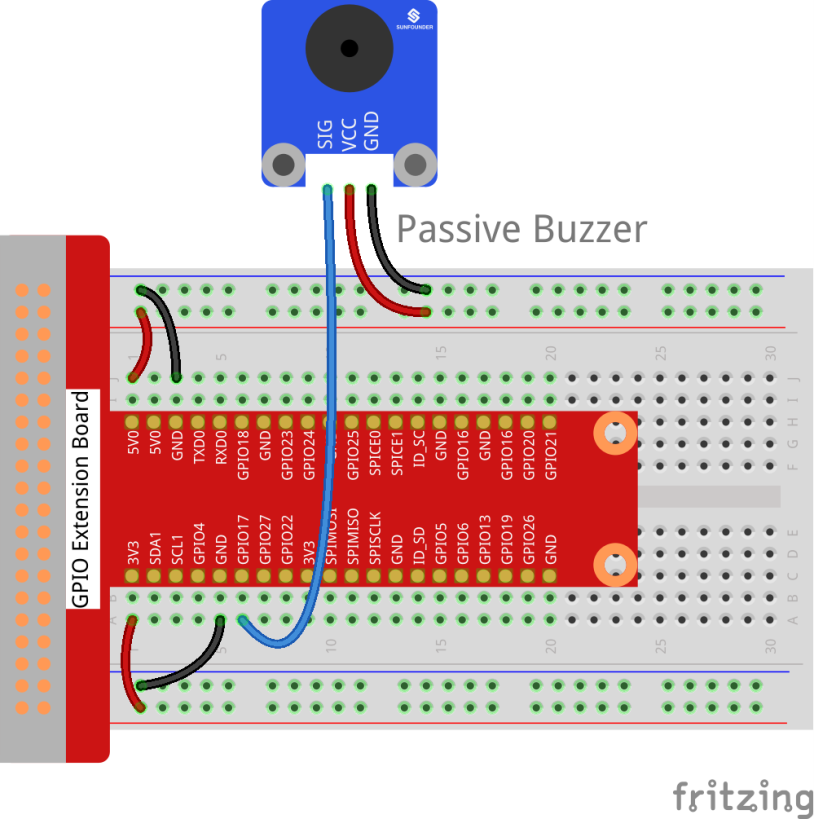
\includegraphics{VerkabelungAkustik}
  \caption{Verkabelung Buzzer}
  \label{fig:Buzzer}
\end{figure}

\begin{table}[] \centering
\begin{tabular}{lll}
Bezeichnung     & GPIO Bus & Buzzer \\ \hline
Stromversorgung & 3V3      & VCC    \\
Ground          & GND      & GND    \\
Signal          & GPIO17   & SIG
\end{tabular}
\end{table}

Über den GPIO Bus des Raspberry Pi kann der Buzzer direkt angesprochen und versorgt werden. Ein einzelnes Signalkabel reicht für die Kommunikation aus und hält den Aufbau weitestgehend simpel.

\subparagraph{Daten}
Dem Buzzer werden verschiedene Frequenzen gesendet, welche dieser dementsprechend abspielt. Somit ist das Spielen einer Melodie möglich. Für unsere Benutzung reicht jedoch eine einzelne Frequenz. Die Frequenz wird im Interval von 500ms an den Buzzer gesendet und ist somit in der Lage das höchste Zahl "9" innerhalb von 4.5s abzuspielen.

Die Freuenz wird in Form einer Zahl gesendet, der Frequenzbereich variert je nach Buzzer.

\paragraph{Realisierung}
Der Code wird in Python realisiert und macht Verwendung von den Bibliotheken GPIO und time. Es wird in einem Interval (500ms) eine Frequenz auf den GPIO Port ausgegeben. Alle Module/Komponente werden asynchron ausgeführt, das Ausführen von time.sleep(ms) sollte somit kein Problem sein.

Das Buzzen wird aus einer selbstimplementierten "Sound" Bibliothek über die Funktion "buzz\_by\_number(number)" ausgeführt. Dabei wird über eine Schnittstelle das gewünschte Signal an den Buzzer gesendet.


\end{document}
